\documentclass[a4paper,UKenglish,cleveref, autoref, thm-restate]{oasics-v2021}
%This is a template for producing OASIcs articles. 
%See oasics-v2021-authors-guidelines.pdf for further information.
%for A4 paper format use option "a4paper", for US-letter use option "letterpaper"
%for british hyphenation rules use option "UKenglish", for american hyphenation rules use option "USenglish"
%for section-numbered lemmas etc., use "numberwithinsect"
%for enabling cleveref support, use "cleveref"
%for enabling autoref support, use "autoref"
%for anonymousing the authors (e.g. for double-blind review), add "anonymous"
%for enabling thm-restate support, use "thm-restate"
%for enabling a two-column layout for the author/affilation part (only applicable for > 6 authors), use "authorcolumns"
%for producing a PDF according the PDF/A standard, add "pdfa"

%\pdfoutput=1 %uncomment to ensure pdflatex processing (mandatatory e.g. to submit to arXiv)
%\hideOASIcs %uncomment to remove references to OASIcs series (logo, DOI, ...), e.g. when preparing a pre-final version to be uploaded to arXiv or another public repository

%\graphicspath{{./graphics/}}%helpful if your graphic files are in another directory
\usepackage{lmodern}
\usepackage{graphicx}
\usepackage{booktabs}
\usepackage{wrapstuff}
\usepackage{numprint}
\usepackage{wrapfig}
\usepackage{amsfonts}
\usepackage{mathpartir}
\usepackage{tikz}
\usepackage{mystyle}
\usepackage{upquote}
\bibliographystyle{plainurl}% the mandatory bibstyle

\title{Isabelle/Solidity for Smart Contracts} %TODO Please add

%\titlerunning{Dummy short title} %TODO optional, please use if title is longer than one line

\author{Jane {Open Access}}{Dummy University Computing Laboratory, [optional: Address], Country \and My second affiliation, Country \and \url{http://www.myhomepage.edu} }{johnqpublic@dummyuni.org}{https://orcid.org/0000-0002-1825-0097}{(Optional) author-specific funding acknowledgements}%TODO mandatory, please use full name; only 1 author per \author macro; first two parameters are mandatory, other parameters can be empty. Please provide at least the name of the affiliation and the country. The full address is optional. Use additional curly braces to indicate the correct name splitting when the last name consists of multiple name parts.

\author{Joan R. Public\footnote{Optional footnote, e.g. to mark corresponding author}}{Department of Informatics, Dummy College, [optional: Address], Country}{joanrpublic@dummycollege.org}{[orcid]}{[funding]}

\authorrunning{J. Open Access and J.\,R. Public} %TODO mandatory. First: Use abbreviated first/middle names. Second (only in severe cases): Use first author plus 'et al.'

\Copyright{Jane Open Access and Joan R. Public} %TODO mandatory, please use full first names. LIPIcs license is "CC-BY";  http://creativecommons.org/licenses/by/3.0/
\ccsdesc[100]{\textcolor{red}{Replace ccsdesc macro with valid one}} %TODO mandatory: Please choose ACM 2012 classifications from https://dl.acm.org/ccs/ccs_flat.cfm 

\keywords{Program Verification, Smart Contracts, Isabelle, Solidity} %TODO mandatory; please add comma-separated list of keywords

\category{} %optional, e.g. invited paper

\relatedversion{} %optional, e.g. full version hosted on arXiv, HAL, or other respository/website
%\relatedversiondetails[linktext={opt. text shown instead of the URL}, cite=DBLP:books/mk/GrayR93]{Classification (e.g. Full Version, Extended Version, Previous Version}{URL to related version} %linktext and cite are optional

%\supplement{}%optional, e.g. related research data, source code, ... hosted on a repository like zenodo, figshare, GitHub, ...
%\supplementdetails[linktext={opt. text shown instead of the URL}, cite=DBLP:books/mk/GrayR93, subcategory={Description, Subcategory}, swhid={Software Heritage Identifier}]{General Classification (e.g. Software, Dataset, Model, ...)}{URL to related version} %linktext, cite, and subcategory are optional

%\funding{(Optional) general funding statement \dots}%optional, to capture a funding statement, which applies to all authors. Please enter author specific funding statements as fifth argument of the \author macro.

\acknowledgements{I want to thank \dots}%optional

%\nolinenumbers %uncomment to disable line numbering

%Editor-only macros:: begin (do not touch as author)%%%%%%%%%%%%%%%%%%%%%%%%%%%%%%%%%%
\EventEditors{John Q. Open and Joan R. Access}
\EventNoEds{2}
\EventLongTitle{42nd Conference on Very Important Topics (CVIT 2016)}
\EventShortTitle{CVIT 2016}
\EventAcronym{CVIT}
\EventYear{2016}
\EventDate{December 24--27, 2016}
\EventLocation{Little Whinging, United Kingdom}
\EventLogo{}
\SeriesVolume{42}
\ArticleNo{23}
%%%%%%%%%%%%%%%%%%%%%%%%%%%%%%%%%%%%%%%%%%%%%%%%%%%%%%

\begin{document}

\maketitle

%TODO mandatory: add short abstract of the document
\begin{abstract}

\end{abstract}

\section{Introduction}
\label{sec-intro}

\section{Overview}
\begin{figure}[!h]
\centering
%\begin{tikzpicture}[show background grid]
\begin{tikzpicture}[]
%PICTURE SCOPE or REFERENCEs
\node at (0, 0) (topleft) [circle] {};
%\node at (11.75, 0) (topright) [circle, draw=red, fill=red] {};
\node (topright) [circle, xshift = 10.5cm, right of = topleft] {};
\node (bottomleft) [circle, yshift = -7.25cm, below of = topleft] {};
\node (bottomright) [circle, xshift = 11.5cm, yshift = -7.25cm, below of = topleft] {};
%\draw (0,-3) [draw=red, fill=red]  -- (5, -4); % CHECK once of the grid is affecting the placement of the objects
%GRID

 \draw (2, -0.45 ) [rounded corners = 4pt, draw=black, fill=blue!4]  -- ++(8.15cm, 0) node[below left] {\textcolor{blue}{\scriptsize{Isabelle/Soildity}}}  --++(0, -5.5cm) --++(-8.15, 0)--cycle;
\draw (2, -0.35 ) [rounded corners = 4pt, draw=black, fill=red!4]  -- ++(8.18cm, 0)  --++(0, 1.3cm) --++(-8.15, 0)node[below right, xshift=2.8cm] {\textcolor{red}{\scriptsize Solidity (v 0.8.25)}}-- cycle;
%\draw (2.5, -0.65) [rounded corners = 4pt, draw=black, fill=blue!4]  -- ++(5cm, 0) --++(0, -2.65cm)--++(-5, 0)--cycle;
%\draw (2.65, -0.85) [rounded corners = 4pt, draw=black, fill=blue!4]  -- ++(3.1cm, 0) --++(0, -2.3cm)--++(-3.1, 0)--cycle;
%INPUTS
%\node (solidity) [thin, draw=black, fill=red!4,  rectangle, rounded corners= 2pt, xshift = 4.40cm, right of = topleft, inner sep = 4pt] {\scriptsize Solidity (v 0.8.25)};
\node (model) [thin, draw=black, fill=red!4,  minimum height= 0.6cm, rectangle, rounded corners= 2pt, xshift = 1.65cm, yshift = 0.10cm, right of = topleft, inner sep = 4pt] {\scriptsize Model};
\node (spec) [thin, draw=black, fill=red!4,  minimum height= 0.6cm, rectangle, rounded corners= 2pt, xshift = 3.40cm, yshift = 0.10cm, right of = topleft, inner sep = 4pt] {\scriptsize Specifications};
\node (ver) [thin, draw=black, fill=red!4,  minimum height= 0.6cm, rectangle, rounded corners= 2pt, xshift = 6.850cm, yshift = 0.10cm, right of = topleft, inner sep = 4pt] {\scriptsize{ Verification Condition Generator}};
\node (sm) [thin, draw=black, fill=blue!4,  rectangle, minimum width=2.3cm, rounded corners= 2pt, xshift = 2.85cm, yshift = -1.25cm, right of = topleft, inner sep = 4pt, align = center] {\scriptsize Isabelle/HOL};
\node (sm1) [thin, draw=black, fill=blue!4,  rectangle, minimum width=2.3cm,  xshift = 2.85cm, yshift = -2.10cm, right of = topleft, inner sep = 2pt, align = center] {\scriptsize{ State.thy,} \\[0.15] \scriptsize{State\_monad.thy,} \\[0.15] \scriptsize{Solidity.thy}};
%
%MODEL TO SM
%\draw  [draw=black, line width = 1.5pt, ->] (model.south)  to [out=270, in=90] (sm.north);; ;;
\draw  [draw=black, line width = 1.5pt, ->] (model.south)  --++(0, -0.35cm) |- (3.25cm, -0.65cm) -| (sm.north);; ;;
%%SM TO HOL CORE
\draw  [draw=black, line width = 1.5pt, <->] (sm.east)  -- ++(3.35cm, 0);;;; ;;
%
\node (dtl) [thin, draw=black, fill=blue!4,  rectangle, minimum width=4.9cm, rounded corners= 2pt, xshift = 7.90cm, yshift = -3.35cm, right of = topleft, inner sep = 4pt, align = center, rotate=90] { {\scriptsize \textcolor{white}{Isabelle/HOL}}\\[0.15] {\scriptsize \textcolor{white}{ Definitions/Theorems/Lemmas}}};
\node (dtl) [thin, draw=black, fill=blue!4,  rectangle, minimum width=4.9cm, rounded corners= 2pt, xshift = 8cm, yshift = -3.45cm, right of = topleft, inner sep = 4pt, align = center, rotate=90] { {\scriptsize Isabelle/HOL}\\[0.15] {\scriptsize  Definitions/Thoerems/Lemmas}};
\node (isac) [thin, draw=black, fill=blue!4,  rectangle, rounded corners= 2pt, minimum width= 5.5cm, xshift = 9.75cm,  yshift= -3.2cm, right of = topleft,  inner sep = 4pt,   align = center, rotate=90] { {\scriptsize Isabelle/HOL Core}};
\draw  [draw=black, line width = 1.5pt, <->] (9.52, -3) -- ++(0.95cm, 0) ;;
%%THEORIES-step02

\node (isasol) [thin, draw=black, fill=blue!4,  rectangle, minimum width=2.3cm, rounded corners= 2pt, xshift = 4.550cm, yshift = -3.55cm, right of = topleft, inner sep = 4pt, align = center] {\scriptsize Isabelle/ML};
\node (isasol1) [thin, draw=black, fill=blue!4,  rectangle, minimum width=2.3cm,  xshift = 4.550cm, yshift = -4.05cm, right of = topleft, inner sep = 4pt, align = center] {\scriptsize{ Contract.thy}};
%SPECIFICATION TO CONTRACT
\draw  [draw=black, line width = 1.5pt, ->] (spec.south)  --++(0, -0.35cm) |- (5.25cm, -0.65cm) -| (isasol.north);; ;;
%%Contract to Modeling
\draw  [draw=black, line width = 1.5pt, <->]  (sm1.south east) --++ (0, -0.5);;
\draw  [draw=black, line width = 1.5pt, ->] (isasol.east) -- ++(1.65cm, 0);;
%
%
%
\node (sc) [thin, draw=black, fill=red!4,  rectangle, rounded corners= 2pt, xshift= -0.75cm, yshift = -3.55cm, right of = topleft, inner sep = 4pt, align = center] {\scriptsize Smart Contract  \&\\[0.05pt] \scriptsize Property Specification };
\draw  [draw=black, line width = 1.5pt, ->] (sc.east) to [ out=360, in=180] (isasol.west);;
\node (vsc) [thin, draw=black, fill=green!10,  rectangle, rounded corners= 2pt, minimum width= 5.5cm, xshift = 10.75cm,  yshift= -3.2cm, right of = topleft,  inner sep = 4pt,   align = center, rotate=90] { {\scriptsize Verified Smart Contract}};
\draw  [draw=black, line width = 1.5pt, ->] (11.01, -3) -- ++(0.5cm, 0) ;;
\node (vcg) [thin, draw=black, fill=blue!4,  rectangle, minimum width=2.3cm, rounded corners= 2pt, xshift = 5.90cm, yshift = -5.10cm, right of = topleft, inner sep = 4pt, align = center] {\scriptsize \scriptsize Isabelle/HOL};

\node (vcg1) [thin, draw=black, fill=blue!4,  rectangle, minimum width=2.3cm, xshift = 5.90cm, yshift = -5.60cm, right of = topleft, inner sep = 4pt, align = center] {\scriptsize{ WP.thy}};


%%CONNECTIONS
%

\node (scp) [thin, draw=black, fill=red!4,  rectangle, rounded corners= 2pt, xshift = -0.80cm, yshift = -5.50cm, right of = topleft, inner sep = 4pt, align = center] {\scriptsize Automatic  Verification};
%
%scp to verification generator
\draw  [draw=black, line width = 1.5pt, <-]  (vcg1.west) --++ (-4.0cm, 0);;
%vcg to modeling
\draw  [draw=black, line width = 1.5pt, <->]  (vcg.west) --++(-1.8cm, 0) -| (sm1.south);;
%Contract to verification generator
\draw  [draw=black, line width = 1.5pt, <->]  (vcg.north west) --++ (0, 0.5);;
%

%WP to VCG
\draw  [draw=black, line width = 1.5pt, <-] (vcg.north)  --++(0, 4.63cm) ;; ;;

\end{tikzpicture}

\end{figure}
\label{sec-ov}

\section{Case Study}
\begin{solidity}{label={fig:casino}}{Solidity source code for the Casino}
	contract Casino {
		enum Coin { HEADS, TAILS } ;
		enum State { IDLE, GAME_AVAILABLE,  BET_PLACED }
		State private state; 
		address public operator, player;
		uint public pot;
		bytes32 public hashedNumber;
		uint public bet;
		Coin guess;

		function createGame(bytes32 hashNum) 
			public byOperator, inState(IDLE) { 
			hashedNumber = hashNum; 
			state = GAME_AVAILABLE;
		}

		function placeBet(Coin _guess) public payable inState(GAME_AVAILABLE) {
			require (msg.sender != operator);
			require (msg.value <= pot);
			state = BET_PLACED; 
			player = msg.sender; 
			bet = msg.value; 
			guess = _guess; 
		}

 		function decideBet(uint secretNumber) 
		public byOperator, inState(BET_PLACED) { 
			require (hashedNumber == keccak256(secretNumber)); 
			Coin secret = (secretNumber \% 2 == 0)? HEADS : TAILS;
			if (secret == guess) {
				pot = pot - bet;  
				player.transfer(bet*2);  bet = 0;} 
			else {
				pot = pot + bet; bet = 0;
				}
			state = IDLE;}
		function addToPot() public payable byOperator { pot = pot + msg.value;}

		function removeFromPot(uint amount) public byOperator, noActiveBet { 
			operator.transfer(amount);  
			pot = pot - amount;}
		}
\end{solidity}
%% ADD LINE NUMBERS;
%% ADD LOGIC OF CODE WHERE NECESSARY
Casino (Listing \ref{fig:casino}) implements a bet game based on the flip-coin (Line 2) using Solidity syntex. 
%
This game has three explicit state: \texttt{IDLE}, \texttt{GAME\_AVAILABLE}, \texttt{BET\_PLACED} (Line 3).
%
An operator may create a new game by calling \texttt{creatGame} function (Line 11-15).
%
The operator provides a \texttt{hashNum} (Line 11) to ensure unbiased and verifiable bet (Line 26-30).
%
The function,  \texttt{creatGame}, uses two modifiers (\texttt{byOperator} and \texttt{inState(s)}) to implement only operator access and state-flow control, i.e., new game can only be created in \texttt{IDLE} state.
%
The \texttt{creatGame} function  changes the state to \texttt{BET\_PLACED} which allows players to place bet on \texttt{HEADS} or \texttt{TAILS}, as \texttt{\_guess}, by calling \texttt{betPlaced} function.
%
The \texttt{betPlaced} function uses \texttt{require} to safe guard possible manipulation from operator by restricting its access (Line 18) and payout safety by capping the maximum bet amount with pot balance (Line 19) in the game.
%

%
Once the game is in \texttt{BET\_PLACED}, the operator may decide the bet (\texttt{decideBet}) by passing \texttt{secretNumber} (Line 26). The secret number is used to verify the bet against \texttt{hashNumber} (Line 28) to ensure fairness. 
%
Then, secret number is used to reveal \texttt{HEADS} (even) or \texttt{TAILS} (odd) (Line 29) which is further utilized to resolve the bet (Line 30-33).
%
In case, player wins,  then double amount of the original bet is transferred to the player's account (Line 30), otherwise, amount equivalent to original bet is added to the pot (Line 32). 
%

%
Finally, in \texttt{IDLE} and \texttt{GAME\_AVAILABLE} states, an operator may add or remove any amount of money from pot  by invoking \texttt{addToPot} or \texttt{removeFromPot} function.
%%
However, in \texttt{BET\_PLACED} state, an operator is allowed to only remove the money which is ensured by the modifier \texttt{noActiveBet}.
%
%
%\vspace{-0.25cm}
\section{Specification}
In this section, we present a Solidity equivalent specification of smart contracts in Isabelle/Solidity. 
%
We primarly focused on specifications of state or local variables, data types, functions, modifiers, precondition specifiers and statments in Isabelle/Solidity.
%\vspace{-1cm}
\paragraph*{Storage Variables}
%
%Our tool facilitates the specification of a contract using Isabelle/Solidity command \texttt{\color{isacom}contract} followed by \emph{name} and list of storage variables.
%
%The tool allows data-type annotations to specify \texttt{Casino} stroage variables  (Listing \ref{fig:isadt}).
In Listing \ref{fig:isadt}, Casino smart contract is defined using Isabelle/Solidity command \texttt{\color{isacom}contract} followed by \emph{name} and list of storage variables.
%
The tool, also,  allows data-type annotations to specify the types of variables (Listing \ref{fig:isadt}).
\begin{isabelle}{label={fig:isadt}}{Isabelle/Solidity data types for Casino}
contract Casino
  	for "STR state": TSint
  	and "STR operator": TAddress
 	and "STR player": TAddress
  	and "STR pot": TSint
  	and "STR hashedNumber": TBytes
  	and "STR bet": TSint
  	and "STR guess": TSint
\end{isabelle}
%
%\begin{center}
%		\fbox{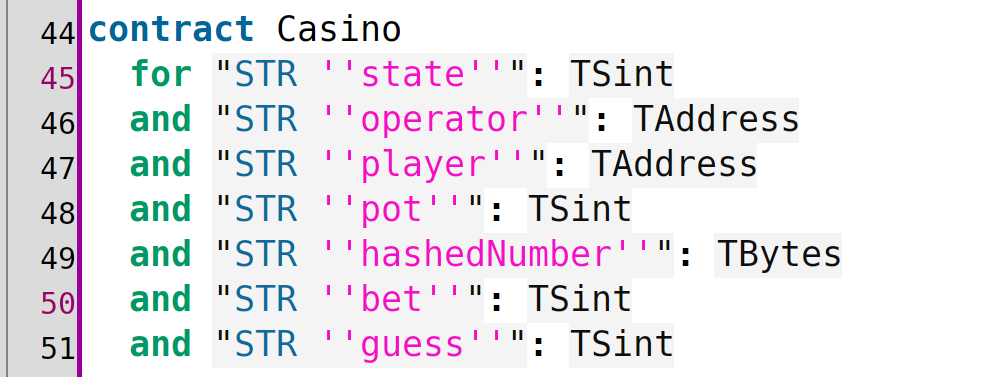
\includegraphics[width=.5\textwidth]{sc-dt.png}}
%	\end{center}
%\begin{Example}{}{Storage Variables}
%	
%	\begin{center}\vspace{-2mm}
%		\fbox{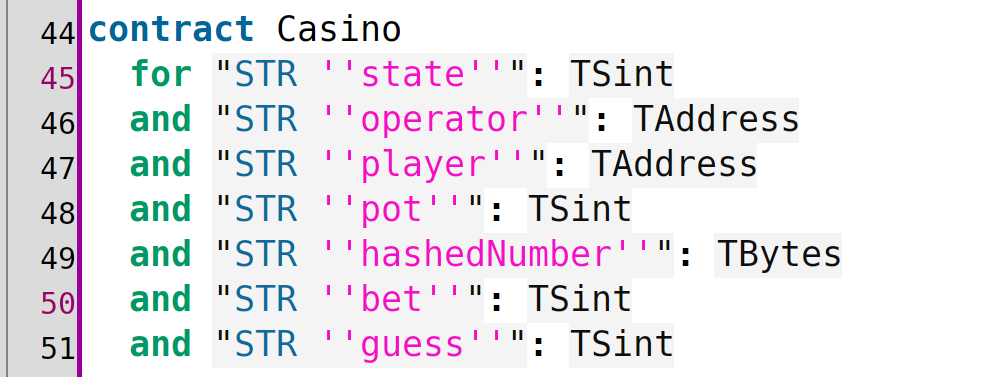
\includegraphics[width=.45\textwidth]{sc-dt.png}}
%	\end{center}\vspace{-2mm}
%	\end{Example}
%
\paragraph*{Methods}
%For Solidity functions, Isabelle/Solidity uses keyword \texttt{\color{isargreen}emethod} followed by \emph{name} and modifier \texttt{\color{isargreen}payable}.
%
%Isabelle/Solidity allows declaring memory variables for functions using keyword \texttt{\color{isargreen}param}.
%
%The body of the funciton is formally specified using  \texttt{\color{isargreen}where} \texttt{"do \{\dots\}",} structure.
%
%
%The keyword \texttt{\color{isargreen}param} specifies a memory (local) variable, \texttt{amount}, of type integer.
%
 %
%
%
%The k
A function, \texttt{removeFromPot}, in Listing \ref{fig:isamethod} showcases Isabelle/Solidity features to specify Solidity functions.
%
The keyword \texttt{\color{isargreen}emethod} defines \texttt{removeFromPot} which has a \texttt{\color{isargreen}payable}  modifier. 
%
A memory (local) variable, \texttt{amount}, of  integer type for the function is declared using keyword  \texttt{\color{isargreen}param}.
%
Isabelle/Solidity allows to specify the body of the function using \texttt{\color{isargreen}where} \texttt{"do \{\dots\}",} structure.
%
%
\begin{isabelle}{label={fig:isamethod}}{Isabelle/Solidity method for Casino}
emethod removeFromPot payable
  param "STR amount": TSint
where
  "do {
    byOperator;
    noActiveBet;
    assign_storage_monad (STR ''pot'') [] 
	(minus_monad_safe (storeLookup (STR ''pot'') []) 
		(stackLookup (STR ''amount'') []));
    transfer_monad (storeLookup (STR ''operator'') []) 
	(stackLookup (STR ''amount'') [])
  }"
\end{isabelle}
%

%
Preconditions on access control, \texttt{byOperator}, and state-flow, \texttt{noActiveBet}, are specified as constants which are based on a higher-order logic funciton, i.e., \texttt{assert}, given in Listing \ref{def:assert}. 
%
The function \texttt{assert} returns normal exection if \texttt{msg.sender} is the operator else it throws an exception.
%
In this way, Isabelle/Solidity ensures the preconditions which ensures intended behavior of the method.
%
\begin{isabelle}{label={def:assert}}{Preocndition in Isabelle/Solidity}
abbreviation byOperator::"(unit, ex, 'a state) state_monad" where
 "byOperator $\equiv$ assert Err ($\lambda$s. sdata.Value (valtype.Address msg_sender)
			 = state.Storage s this (STR ''operator''))"
\end{isabelle}

Isabelle/Solidity also supports Solidity statements such as control structures and assignment operators. 
%
From Line 7-9, an \texttt{amount} is subtracted from the \texttt{pot} using \texttt{assign\_storage} \texttt{\_monad} which besides identifiers also need store location depending on the variable type.
%

%
Next, 
%
in Line 10 (of Listing \ref{fig:isamethod}), \texttt{transfer\_monad} transfers (special function) an amount  equal to the bet is transferred to the operator account.
\section{Verification}
%
%
%
Isabelle/Solidity facilitates invariance specification using \texttt{\color{isarblue}invariant} command over the contract balance and storage.
%
This command requires a user to provide the name of the invariant, followed by the invariant as predicates formulated over the contracts. The command then generates introduction and elimination rules which can be invoked for automated verification of the invariants.
%
\begin{Example}{Invariant}{invariant}
	Assume that we want to verify that when game is in  \texttt{BET\_PLACED} state, contract internal balance satisfies:
	\begin{equation}
		(s(\STR{balances})) \ge pot + bet  \wedge bet \leq pot
	\end{equation}\label{eq:inv}
	and if not in \texttt{BET\_PLACED}, then 
\begin{equation}
		(s(\STR{balances})) \ge pot 
	\end{equation}\label{eq:inv1}
Above invariant enusres payout safety for players. 
%

%
The corresponding specification in Isabelle/Solidity is given in Listing \ref{def:inv}:
\begin{isabelle}{label={def:inv}}{Invariant in Isabelle/Solidity}
invariant pot_balance sb where
    "(fst sb STR ''state'' = sdata.Value (Sint 2)
      $\longrightarrow$ snd sb $\geq$ unat (valtype.sint (sdata.vt (fst sb STR ''pot''))) 
		+ unat (valtype.sint (sdata.vt (fst sb STR ''bet'')))
        $\wedge$ valtype.sint (sdata.vt (fst sb STR ''bet'')) $\leq$ 
		valtype.sint (sdata.vt (fst sb STR ''pot''))) $\wedge$
    (fst sb STR ''state'' $\neq$ sdata.Value (Sint 2)
    $\longrightarrow$  snd sb $\geq$ unat (valtype.sint (sdata.vt (fst sb STR ''pot''))))"
  for "casino"
\end{isabelle}
\end{Example}
%


\section{Related Work}
%
\section{Conclusion}
%%
%% Bibliography
%%
%

%
%% Please use bibtex, 
\nocite{*}
\bibliography{oasics-v2021-sample-article}

%\appendix
%
%\section{Styles of lists, enumerations, and descriptions}\label{sec:itemStyles}
%
%List of different predefined enumeration styles:
%
%\begin{itemize}
%\item \verb|\begin{itemize}...\end{itemize}|
%\item \dots
%\item \dots
%%\item \dots
%\end{itemize}
%
%\begin{enumerate}
%\item \verb|\begin{enumerate}...\end{enumerate}|
%\item \dots
%\item \dots
%%\item \dots
%\end{enumerate}
%
%\begin{alphaenumerate}
%\item \verb|\begin{alphaenumerate}...\end{alphaenumerate}|
%\item \dots
%\item \dots
%%\item \dots
%\end{alphaenumerate}
%
%\begin{romanenumerate}
%\item \verb|\begin{romanenumerate}...\end{romanenumerate}|
%\item \dots
%\item \dots
%%\item \dots
%\end{romanenumerate}
%
%\begin{bracketenumerate}
%\item \verb|\begin{bracketenumerate}...\end{bracketenumerate}|
%\item \dots
%\item \dots
%%\item \dots
%\end{bracketenumerate}
%
%\begin{description}
%\item[Description 1] \verb|\begin{description} \item[Description 1]  ...\end{description}|
%\item[Description 2] Fusce eu leo nisi. Cras eget orci neque, eleifend dapibus felis. Duis et leo dui. Nam vulputate, velit et laoreet porttitor, quam arcu facilisis dui, sed malesuada risus massa sit amet neque.
%\item[Description 3]  \dots
%%\item \dots
%\end{description}
%
%\cref{testenv-proposition} and \autoref{testenv-proposition} ...
%
%\section{Theorem-like environments}\label{sec:theorem-environments}
%
%List of different predefined enumeration styles:
%
%\begin{theorem}\label{testenv-theorem}
%Fusce eu leo nisi. Cras eget orci neque, eleifend dapibus felis. Duis et leo dui. Nam vulputate, velit et laoreet porttitor, quam arcu facilisis dui, sed malesuada risus massa sit amet neque.
%\end{theorem}
%
%\begin{lemma}\label{testenv-lemma}
%Fusce eu leo nisi. Cras eget orci neque, eleifend dapibus felis. Duis et leo dui. Nam vulputate, velit et laoreet porttitor, quam arcu facilisis dui, sed malesuada risus massa sit amet neque.
%\end{lemma}
%
%\begin{corollary}\label{testenv-corollary}
%Fusce eu leo nisi. Cras eget orci neque, eleifend dapibus felis. Duis et leo dui. Nam vulputate, velit et laoreet porttitor, quam arcu facilisis dui, sed malesuada risus massa sit amet neque.
%\end{corollary}
%
%\begin{proposition}\label{testenv-proposition}
%Fusce eu leo nisi. Cras eget orci neque, eleifend dapibus felis. Duis et leo dui. Nam vulputate, velit et laoreet porttitor, quam arcu facilisis dui, sed malesuada risus massa sit amet neque.
%\end{proposition}
%
%\begin{conjecture}\label{testenv-conjecture}
%Fusce eu leo nisi. Cras eget orci neque, eleifend dapibus felis. Duis et leo dui. Nam vulputate, velit et laoreet porttitor, quam arcu facilisis dui, sed malesuada risus massa sit amet neque.
%\end{conjecture}
%
%\begin{observation}\label{testenv-observation}
%Fusce eu leo nisi. Cras eget orci neque, eleifend dapibus felis. Duis et leo dui. Nam vulputate, velit et laoreet porttitor, quam arcu facilisis dui, sed malesuada risus massa sit amet neque.
%\end{observation}
%
%\begin{exercise}\label{testenv-exercise}
%Fusce eu leo nisi. Cras eget orci neque, eleifend dapibus felis. Duis et leo dui. Nam vulputate, velit et laoreet porttitor, quam arcu facilisis dui, sed malesuada risus massa sit amet neque.
%\end{exercise}
%
%\begin{definition}\label{testenv-definition}
%Fusce eu leo nisi. Cras eget orci neque, eleifend dapibus felis. Duis et leo dui. Nam vulputate, velit et laoreet porttitor, quam arcu facilisis dui, sed malesuada risus massa sit amet neque.
%\end{definition}
%
%\begin{example}\label{testenv-example}
%Fusce eu leo nisi. Cras eget orci neque, eleifend dapibus felis. Duis et leo dui. Nam vulputate, velit et laoreet porttitor, quam arcu facilisis dui, sed malesuada risus massa sit amet neque.
%\end{example}
%
%\begin{note}\label{testenv-note}
%Fusce eu leo nisi. Cras eget orci neque, eleifend dapibus felis. Duis et leo dui. Nam vulputate, velit et laoreet porttitor, quam arcu facilisis dui, sed malesuada risus massa sit amet neque.
%\end{note}
%
%\begin{note*}
%Fusce eu leo nisi. Cras eget orci neque, eleifend dapibus felis. Duis et leo dui. Nam vulputate, velit et laoreet porttitor, quam arcu facilisis dui, sed malesuada risus massa sit amet neque.
%\end{note*}
%
%\begin{remark}\label{testenv-remark}
%Fusce eu leo nisi. Cras eget orci neque, eleifend dapibus felis. Duis et leo dui. Nam vulputate, velit et laoreet porttitor, quam arcu facilisis dui, sed malesuada risus massa sit amet neque.
%\end{remark}
%
%\begin{remark*}
%Fusce eu leo nisi. Cras eget orci neque, eleifend dapibus felis. Duis et leo dui. Nam vulputate, velit et laoreet porttitor, quam arcu facilisis dui, sed malesuada risus massa sit amet neque.
%\end{remark*}
%
%\begin{claim}\label{testenv-claim}
%Fusce eu leo nisi. Cras eget orci neque, eleifend dapibus felis. Duis et leo dui. Nam vulputate, velit et laoreet porttitor, quam arcu facilisis dui, sed malesuada risus massa sit amet neque.
%\end{claim}
%
%\begin{claim*}\label{testenv-claim2}
%Fusce eu leo nisi. Cras eget orci neque, eleifend dapibus felis. Duis et leo dui. Nam vulputate, velit et laoreet porttitor, quam arcu facilisis dui, sed malesuada risus massa sit amet neque.
%\end{claim*}
%
%\begin{proof}
%Fusce eu leo nisi. Cras eget orci neque, eleifend dapibus felis. Duis et leo dui. Nam vulputate, velit et laoreet porttitor, quam arcu facilisis dui, sed malesuada risus massa sit amet neque.
%\end{proof}
%
%\begin{claimproof}
%Fusce eu leo nisi. Cras eget orci neque, eleifend dapibus felis. Duis et leo dui. Nam vulputate, velit et laoreet porttitor, quam arcu facilisis dui, sed malesuada risus massa sit amet neque.
%\end{claimproof}

\end{document}
